\textbf{Agenda}

Pada bab ini kita akan membahas beberapa topik yang berhubungan dengan Control statement yaitu:

\minitoc

Aliran program tidak selalu berjalan secara sekuensial berurutan dari
atas ke bawah, kadang-kadang diperlukan \textbf{percabangan} atau
\textbf{perulangan} atau kombinasi dari keduanya. Semua bahasa
pemrograman mempunyai struktur kendali (\emph{control statement})
demikian juga bahasa C++. Struktur kendali merupakan pengatur aliran
program, mempunyai rangkaian perintah yang harus ditulis untuk memenuhi
beberapa keadaan, yaitu:

\begin{itemize}

\item
  Mengulang suatu perintah jika suatu kondisi dipenuhi.
\item
  Melanjutkan sebuah pernyataan bila kondisi terpenuhi.
\item
  Memilih sebuah pilihan dari beberapa alternatif bila kondisi
  terpenuhi.
\end{itemize}

\section{Percabangan}\label{percabangan}

Adalah perintah yang memungkinkan pemilihan atas perintah yang akan
dijalankan sesuai dengan kondisi tertentu. Ada tiga macam perintah
percabangan dalam C++, yaitu \texttt{if}, \texttt{if\ \ldots{}\ else},
dan \texttt{switch}. Dengan percabangan, suatu baris program akan
dikerjakan jika suatu kondisi dipenuhi (benar) atau tidak (else), jadi
tidak semua baris program akan dieksekusi.

\subsection{Percabangan dengan if}\label{percabangan-dengan-if}

Sintaks penulisannya sebagai berikut:

\begin{lstlisting}[language=c++, numbers=none]
 if (<ekspresi_boolean>)
 {
 <statements>
 }
\end{lstlisting}

Flowchart untuk statment percabangan if seperti pada gambar berikut


\begin{tikzpicture}[node distance = 2cm, auto]
\node [ling] (init){start};
\node [decision, below of=init] (decide) {\textless{}ekspresi \_bool\textgreater{}};
\node [block, below of=decide, node distance=3cm] (statement) {Statement};
\node [ling, below of=statement] (stop) {stop};

%garis
\path [line] (init) -- (decide);
\path [line] (init) -- (decide);
\path [line] (decide) -- node {Yes}(statement);
%\path [line] (statement) |- node [near start] {No} (decide);
\path[line] (statement) -- (stop);
\end{tikzpicture}


\subsection*{Contoh percabangan dengan if}

\begin{enumerate}
	\item  Buka Qt Creator dan buat project Qt Console Application baru dengan
	nama contoh , kemudian tulis kode berikut.
	
	\lstinputlisting[language=c++, caption=percabangan dengan if, label=contoh2-3]{../code/contoh2-3.cpp}
	
	\item  Kemudian jalankan kode diatas dengan menekan tombol Ctrl + R, outputnya adalah sebagai berikut.
	
\begin{lcverbatim}
Masukan nomor: 15
15 lebih besar dari 10
\end{lcverbatim}
\end{enumerate}
\subsection{Percabangan dengan if \dots else}\label{percabangan-dengan-if-..-else}

Sintaks penulisannya sebagai berikut :

\begin{lstlisting}[language=c++]
 if (<ekspresi_boolean>)
 {
 <dijalankan jika ekspresi_boolean benar>
 }
 else
 {
 < dijalankan jika ekspresi_boolean salah>
 }
\end{lstlisting}

Flowchart untuk statment ini adalah :

\begin{quotation}
 {\LARGE \ding{45}} \textbf{CATATAN} 

Di
dalam \texttt{if()} maupun di dalam else bisa diisi dengan perintah
I\textgreater{} \texttt{if()} lagi. Bentuk \texttt{if()} dalam
\texttt{if()} ini sering disebut I\textgreater{} dengan
\texttt{nested\ if} (if bersarang).
\end{quotation}

\begin{tikzpicture}[node distance = 2cm, auto]
\node [ling] (init){start};
\node [decision, below of=init, node distance=2cm] (decide) {\textless{}ekspresi \_bool\textgreater{}};
\node [block, below of=decide, node distance=3cm] (statement) {Statement};
\node [block, right of=decide, node distance=3cm] (statement2) {Statement2};
\node [ling, below of=statement, node distance=2cm] (stop) {stop};

%garis
\path [line] (init) -- (decide);
\path [line] (init) -- (decide);
\path [line] (decide) -- node {Ya}(statement);
%\path [line] (statement) |- node [near start] {No} (decide);
\path[line] (statement) -- (stop);
\path[line] (statement) -| node {tidak}(statement2);
\path[line] (statement2) -- (decide);
\end{tikzpicture}

\subsubsection*{contoh program untuk percabagan if \dots else}

\begin{enumerate}
\item Edit contoh \ref{contoh2-3} dengan menambahkan kode berikut ini

\lstinputlisting[language=c++, firstline=13, lastline=14, caption=percabagan if \dots else, label=contoh2-4]{../code/contoh2-4.cpp}

\item  Kemudian jalankan kode diatas dengan menekan tombol Ctrl + R, outputnya adalah sebagai berikut.

\begin{lcverbatim}
Masukan nomor: 4
4 kurang besar dari 10
\end{lcverbatim}
\end{enumerate}

\subsection{Percanbangan dengan if bersarang}

Flowchart untuk statment if bersarang ini adalah :

\begin{tikzpicture}[node distance = 1cm, auto]
\node [ling] (init){start};
\node [decision, below of=init, node distance=3cm] (decide) {\textless{}ekspresi \_bool\textgreater{}};
\node [block, below of=decide, node distance=3cm] (statement) {Statement};

\node [decision, right of=decide, node distance=3cm] (decide1) {\textless{}ekspresi \_bool\textgreater{}};
\node [block, below of=decide1, node distance=3cm] (statement1) {Statement1};

\node [block, right of=decide1, node distance=6cm] (statement2) {Statement2};
\node [ling, below of=statement, node distance=2cm] (stop) {stop};

%garis
\path [line] (init) -- (decide);
\path [line] (decide) -- node{Tidak}(decide1);
\path [line,dashed](decide1) -- node{tidak\dots dst \dots tidak }(statement2);
\path [line] (decide) -- node{Ya}(statement);
\path [line] (decide1) -- node {Ya} (statement1);
\path[line] (statement) -- (stop);

\path[line] (statement2) |- (stop);
\path[line] (statement1) |- (stop);
\path [line] (decide) -- node {Ya}(statement);

\end{tikzpicture}

\subsection{Percabangan dengan switch}\label{percabangan-dengan-switch}

Perintah ini digunakan sebagai alternatif pengganti dari statment
\texttt{if\ \ldots{}\ else} dengan \texttt{else} lebih dari satu. Dengan
perintah ini percabangan dapat diarahkan pada beberapa alternatif
pilihan berdasarkan nilai ekspresi. Berbeda dengan \texttt{if},
\texttt{switch} tidak dapat medeteksi \emph{operator pembanding}
(\textgreater{}, \textless{}, dsb.), karena ekspresi degan operator ini
menghasilkan nilai \emph{boolean}, melainkan hanya dapat mengalihkan
alur program ke suatu nilai yang sama, pada statement ini ekspresi yang
diminta harus menghasilkan bilangan \emph{bulat}.

\begin{lstlisting}[language=c++, numbers=none]
 switch (<ekspresi>)
 {
 case <konst_1>: <pernyataan_1>;
 break;
 case <konst_2>: <pernyataan_2>;
 break;
 case <konst_n>: <pernyataan_n>;
 break;
 default : <pernyataan_default>;
 }
\end{lstlisting}

Perintah \texttt{switch} akan membaca nilai dari
\texttt{\textless{}ekspresi\textgreater{}} kemudian membandingkan
hasilnya dengan konstanta-konstanta
(\texttt{\textless{}konst\_1\textgreater{}},
\texttt{\textless{}konst\_2\textgreater{}},
\texttt{\textless{}konst\_n\textgreater{}}) yang berada di case.
Pembandingan akan dimulai dari
\texttt{\textless{}konst\_1\textgreater{}} sampai konstanta
\texttt{\textless{}konst\_n\textgreater{}}. Jika hasil dari kondisi sama
dengan nilai konstanta tertentu, misalnya
\texttt{\textless{}konst\_1\textgreater{}}, maka pernyataan 1 akan
dijalankan sampai ditemukan \texttt{break}. Pernyataan \texttt{break}
akan membawa proses keluar dari perintah \texttt{switch}. Jika hasil
dari kondisi tidak ada yang sama dengan konstanta-konstanta yang
diberikan, maka pernyataan pada \emph{default} yang akan dijalankan.

Flowchart untuk statement ini adalah :

\begin{tikzpicture}[node distance = 1cm, auto]
\node [blok] (ekspresi) {\textless{}nilai\_ekspresi1\textgreater{}};
\node [blok,below of=ekspresi] (ekspresi1) {\textless{}nilai\_ekspresi2\textgreater{}};
\node [blok,below of=ekspresi1] (ekspresi2) {\textless{}nilai\_ekspresi3\textgreater{}};
\node [blok,below of=ekspresi2] (ekspresi3) {\textless{}nilai\_ekspresi4\textgreater{}};
\node [blok,below of=ekspresi3, node distance=2cm] (ekspresi4) {\textless{}nilai\_lainya\textgreater{}};

\node [titik, left of=ekspresi2, node distance=2cm] (titik) {};
\node [decision, left of=titik, node distance=2cm] (decide) {\textless{}ekspresi\textgreater{}};

\node [blok, right of=ekspresi, node distance=4cm] (statement) {\textless{}statement1\textgreater{}};
\node [blok,below of=statement] (statement1) {\textless{}statement2\textgreater{}};
\node [blok,below of=statement1] (statement2) {\textless{}statement3\textgreater{}};
\node [blok,below of=statement2] (statement3) {\textless{}statement4\textgreater{}};
\node [blok,below of=statement3, node distance=2cm] (statement4) {\textless{}statement\textgreater{}};

\node [ling, above of=decide, node distance=3cm] (start) {start};
\node [ling, right of=statement4, node distance=3cm] (stop) {stop};


\path[line](start) -- (decide);
\path[line](titik) |- (ekspresi);
\path[line](titik) |- (ekspresi1);
\path[line](titik) |- (ekspresi2);
\path[line](titik) |- (ekspresi3);
\path[line](titik) |- (ekspresi4);
\path[line,dashed](ekspresi3) -- node{dst}(ekspresi4);

\path[line](ekspresi) -- (statement);
\path[line](ekspresi1) -- (statement1);
\path[line](ekspresi2) -- (statement2);
\path[line](ekspresi3) -- (statement3);
\path[line](ekspresi4) -- (statement4);
\path[line,dashed](statement3) -- node{dst}(statement4);

\path[line](statement) -| (stop);
\path[line](statement1) -| (stop);
\path[line](statement2) -| (stop);
\path[line](statement3) -| (stop);
\path[line](statement4) -- (stop);

\path[line](decide) -- (titik);
\end{tikzpicture}



\subsection{Contoh Tipe data dan Identifier.}

\begin{enumerate}

\item
  Buka Qt Creator dan buat project Qt Console Application baru dengan
  nama contoh \ref{contoh2-2}, kemudian tulis kode berikut.

\lstinputlisting[language=c++, caption=Tipe data dan Identifier, label=contoh2-2]{../code/contoh2-2.cpp}


\item
  Kemudian jalankan kode diatas dengan menekan tombol Ctrl+R, outputnya
  adalah sebagai berikut.

 \begin{lcverbatim}
sabtu
\end{lcverbatim}

\end{enumerate}



\subsubsection*{Keterangan Program}

\begin{itemize}

\item
  Pada program di atas variabel \texttt{hari} dideklarasikan bertipe
  \texttt{int} dan diinisialisasi dengan nilai \texttt{6}.
\item
  Kemudian pada bagian ekspresi di dalam \texttt{switch} di isi variabel
  \texttt{hari}, hasil ekspresi tersebut di evaluasi, karena
  menghasilkan nilai 6, maka yang dicetak ke layar adalah
  ``\textbf{Sabtu}''.
\end{itemize}

\section{Perulangan}\label{perulangan}

Perulangan digunakan untuk mengulang suatu perintah sebanyak yang
diinginkan tanpa harus menulis ulang. C++ mengenal tiga jenis perintah
perulangan, yaitu \texttt{for}, \texttt{while} dan \texttt{do\ ..while}.

\subsection{Perulangan dengan for}\label{perulangan-dengan-for}

Digunakan untuk mengulangi perintah dengan jumlah perulangan yang sudah
diketahui. Pada statement for ini perlu dituliskan suatu kondisi untuk
diuji yang berupa ekspresi boolean, nilai awal dan perintah yang dipakai
untuk penghitung (counter). Nilai variabel penghitung akan secara
otomatis bertambah atau berkurang tiap kali sebuah perulangan
dilaksanakan tergantung perintah yang ditulis pada argumen ini.

Bentuk umum penulisannya sebagai berikut :

\begin{lstlisting}[language=c++, numbers=none]
 for(<nilai_awal>; <ekspresi_boolean>; <penambahan/penurunan>)
 {
 <statmemnts>
 }
\end{lstlisting}

\begin{figure}[htbp]
\centering
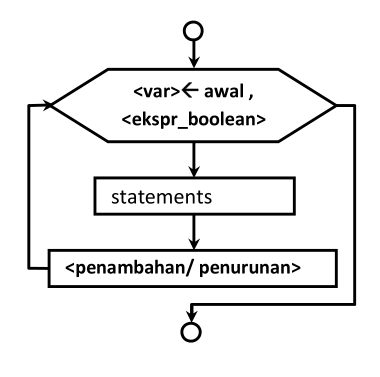
\includegraphics[width=8cm]{Capture2-8}
\caption{flowchart perulangan dengan for}
\end{figure}

\subsection{Perulangan dengan while}\label{perulangan-dengan-while}

Perintah ini digunakan untuk mengulangi suatu perintah sampai kondisi
tertentu. Perulangan akan terus berjalan selama kondisi masih bernilai
benar.

Sintaks penulisannya sebagai berikut :

\begin{lstlisting}[language=c++, numbers=none]
for(<nilai_awal>; <ekspresi_boolean>; <penambahan/penurunan>)
{
<statmemnts>
}
\end{lstlisting}

\begin{figure}[htbp]
\centering
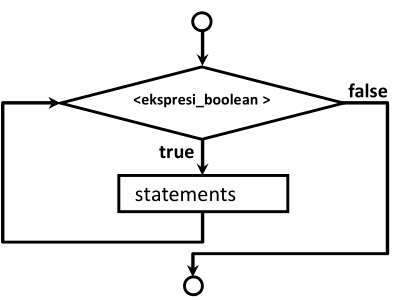
\includegraphics[width=8cm]{Capture2-9}
\caption{flowchart perulangan dengan while}
\end{figure}

\subsection{Perulangan dengan do \dots while}\label{perulangan-dengan-do-while}

Proses perulangan akan berjalan jika kondisi yang diperiksa di
\texttt{while} masih bernilai benar dan perulangan akan dihentikan jika
kondisinya sudah bernilai salah.

Sintaks penulisannya sebagai berikut :

\begin{lstlisting}[language=c++, numbers=none]
 do
 {
 <statements>
 }
 while(<expresi_boolean>)
\end{lstlisting}

\begin{figure}[htbp]
\centering
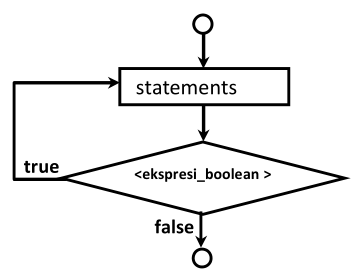
\includegraphics[width=8cm]{Capture2-10}
\caption{flowchart perulangan dengan do\dots while}
\end{figure}

Perbedaan antara perintah \texttt{while} dengan
\texttt{do\ \ldots{}\ while} adalah terletak dari kondisi yang
diperiksa. Pada perintah \texttt{while}, kondisi yang diperiksa terletak
diawal perulangan, sehingga sebelum masuk ke dalam perulangan
\texttt{while} kondisi harus bernilai benar. Sedangkan pada perintah
\texttt{do\ \ldots{}\ while}, kondisi diperiksa di akhir perulangan. Ini
berarti bahwa paling sedikit sebuah perulangan akan dilakukan oleh
perintah \texttt{do\ \ldots{}\ while}, karena untuk masuk ke dalam
perulangan tidak ada kondisi yang harus dipenuhi.

\subsection{Kata kunci continue dan break}\label{kata-kunci-continue-dan-break}

Kata kunci \texttt{break} digunakan untuk keluar dari suatu blok
programn sebelum ekspresi \emph{boloean} yang ada pada statement
tersebut menghentikan, sedangkan kata kunci \texttt{continue} dugunakan
untuk mengabaikan baris perintah suatu perintah di bawahnya dan
melanjutkan ke perulangan selanjutnya.

Sintaks penulisan \texttt{break} dan \texttt{continue} adalah sebagai
berikut :

\begin{lstlisting}[language=c++, numbers=none]
 while(<expresi_boolean1>)
 {
 <statements>
 if(<expresi_boolean2>)
 continue;
 <statements>
 }
\end{lstlisting}